% HC 6001 -- Dr. Castillo -- 31 October 2024
% Transcription of the 12-page handwritten lecture "rotations".
%
% Per-lecture symbol declarations (governed by SYMBOL_CONVENTIONS.md).  The
% shared style file deliberately binds no quantity to a letter; the macros below
% are local to THIS document and exist to make the two decorations that carry the
% most meaning -- the superscript 0 on the space axes and its absence on the body
% axes -- impossible to drop.
\documentclass[11pt]{article}
\usepackage{goldsteinnotes}
\usepackage{xcolor}

% Space (inertial) triad  \ezero{i} = e_i^0   vs.  body triad \ehat{i} = e_i.
\newcommand{\ehat}[1]{\hat{e}_{#1}}
\newcommand{\ezero}[1]{\hat{e}^{\,0}_{#1}}
% Struck-out material inside math.
\newcommand{\mstruck}[1]{\text{\retracted{\ensuremath{#1}}}}
% The lecturer's ink colours (semantic -- see the notes themselves).
\definecolor{lecblue}{RGB}{45,45,200}
\definecolor{lecgreen}{RGB}{0,125,45}
\definecolor{lecred}{RGB}{200,25,25}
\newcommand{\src}[1]{\par\nobreak\vspace{-4pt}\hfill{\footnotesize\itshape[source p.~#1]}\par\nobreak\vspace{2pt}}

\title{Rotations, Non-Inertial Systems, and Rigid Body Motion}
\author{HC 6001 --- Dr.\ Castillo}
\date{31 October 2024}

\begin{document}
\maketitle

\section*{\textcolor{lecblue}{Summary on Elementary Rotations}}
\src{1}

\begin{gather*}
L_z = I\,\omega_z \tag{1}\label{eq:A1}\\[2pt]
\vec{N} = \vec{r}\times\vec{F} \tag{2}\label{eq:A2}\\[2pt]
T = \frac{I}{2}\,\omega_z^{2} \;=\; \frac{\omega_z L_z}{2} \tag{3}\label{eq:A3}
\end{gather*}
\begin{equation*}
\frac{\d\vec{L}}{\d t} = \vec{N}^{(e)}
\qquad
\left\{
\begin{array}{l}
\text{\textsc{inertial frame}}\\[2pt]
\text{\textsc{cm frame} (\textsc{origin at cm, axes parallel to inertial axes})}
\end{array}\right.
\tag{4}\label{eq:A4}
\end{equation*}

\subsection*{Rolling without slipping condition}

\begin{gather*}
v_{\mathrm{CM}\,x} + \omega_z R = 0 \tag{5}\label{eq:A5}\\[2pt]
(\,\omega_z < 0 \text{ for clockwise rotation}\,) \tag{6}\label{eq:A6}
\end{gather*}

\begin{figure}[htbp]
\centering
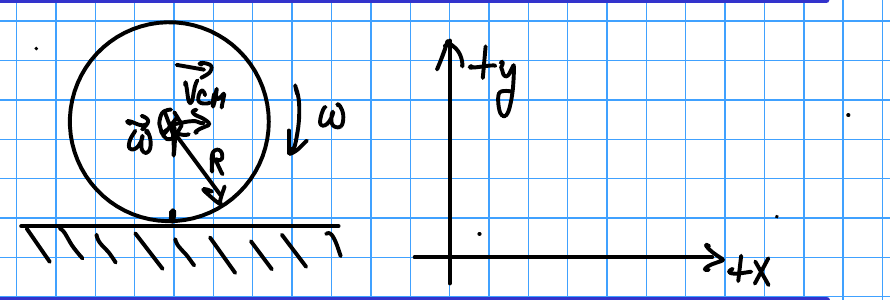
\includegraphics[width=0.72\textwidth]{figures/rot_p1_rolling.png}
\caption{Rolling circle: $\vec{v}_{\mathrm{CM}}$, $\vec{\omega}$ and the radius $R$ to the
contact point, with the sign convention of the $+x$, $+y$ axes drawn alongside.}
\end{figure}

\subsection*{Parallel Axis Theorem}

\begin{gather*}
I = \bar{I} + M a^{2} \tag{7}\label{eq:A7}\\[2pt]
\bar{I} \equiv \text{Moment of inertia around CM} \tag{8}\label{eq:A8}\\[2pt]
a \equiv \text{Distance between axis of rotation and CM} \tag{9}\label{eq:A9}
\end{gather*}

\subsection*{Separating CM Motion}

\begin{align*}
\vec{L} &= \vec{R}\times M\dot{\vec{R}} + \sum_j \vec{r}\,'_j \times m_j\,\dot{\vec{r}}\,'_j
\tag{10}\label{eq:A10}\\[2pt]
T &= \frac{M}{2}\,\bigl|\dot{\vec{R}}\bigr|^{2} + \frac{1}{2}\sum_j m_j \bigl|\dot{\vec{r}}\,'_j\bigr|^{2}
\tag{11}\label{eq:A11}\\[2pt]
M &= \sum_j m_j \tag{12}\label{eq:A12}\\[2pt]
\vec{R} &\equiv \frac{\sum_j m_j \vec{r}_j}{M} \tag{13}\label{eq:A13}\\[2pt]
\vec{r}\,'_j &\equiv \vec{r}_j - \vec{R}
\qquad \text{\textsc{position relative to cm}} \tag{14}\label{eq:A14}
\end{align*}

\begin{figure}[htbp]
\centering
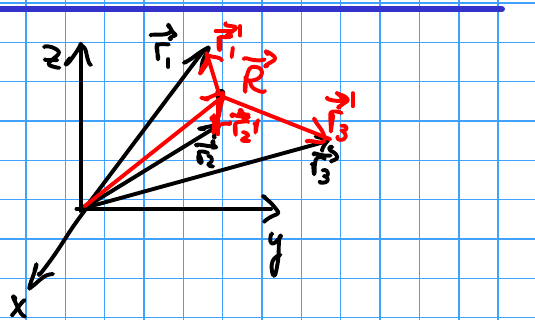
\includegraphics[width=0.48\textwidth]{figures/rot_p1_cmvectors.png}
\caption{Laboratory position vectors $\vec{r}_1,\vec{r}_2,\vec{r}_3$ (black), the centre-of-mass
vector $\vec{R}$ and the relative vectors $\vec{r}\,'_1,\vec{r}\,'_2,\vec{r}\,'_3$ (red).}
\end{figure}

For rigid body, considering rotation with angular velocity $\omega_z$ around CM:
\begin{gather*}
L_z = \bigl(\vec{R}\times M\dot{\vec{R}}\bigr)_z + I\,\omega_z \tag{16}\label{eq:A16}\\[2pt]
T = \frac{M}{2}\bigl|\dot{\vec{R}}\bigr|^{2} + \frac{I}{2}\,\omega_z^{2} \tag{17}\label{eq:A17}
\end{gather*}

\subsection*{\textcolor{lecblue}{Proofs}}

\textsc{changing to cm system:}
\begin{align*}
\vec{L} &= \sum_{i=1}^{N} \vec{r}_i \times m_i \dot{\vec{r}}_i
= \sum_{i=1}^{N}\bigl(\vec{R}+\vec{r}\,'_i\bigr)\times m_i\bigl(\dot{\vec{R}}+\dot{\vec{r}}\,'_i\bigr)\\
&= \sum_i \vec{R}\times m_i \dot{\vec{R}} \;+\; \sum_i \vec{r}\,'_i \times m_i \dot{\vec{r}}\,'_i
\;+\; \text{\textsc{cross-terms}} \tag{18}\label{eq:A18}
\end{align*}
\begin{equation*}
\boxed{\;\vec{r}_i = \vec{R}+\vec{r}\,'_i \qquad \dot{\vec{r}}_i = \dot{\vec{R}}+\dot{\vec{r}}\,'_i\;}
\tag{19}\label{eq:A19}
\end{equation*}

\textsc{cross-terms:}
\begin{align*}
\sum_i \vec{r}\,'_i \times m_i\dot{\vec{R}}
&= \sum_i m_i\bigl(\vec{r}_i-\vec{R}\bigr)\times\dot{\vec{R}}
= \Bigl[\underbrace{\textstyle\sum_i m_i\vec{r}_i}_{M\vec{R}}
- \underbrace{\bigl(\textstyle\sum_i m_i\bigr)\vec{R}}_{M\vec{R}}\Bigr]\times\dot{\vec{R}}\\
&= \bigl[M\vec{R}-M\vec{R}\bigr]\times\dot{\vec{R}} = \vec{0} \tag{20}\label{eq:A20}\\[6pt]
\sum_i \vec{R}\times m_i\dot{\vec{r}}\,'_i
&= \vec{R}\times\sum_i m_i\bigl(\dot{\vec{r}}_i-\dot{\vec{R}}\bigr)
= \vec{R}\times\Bigl[\underbrace{\textstyle\sum_i m_i\dot{\vec{r}}_i}_{M\dot{\vec{R}}}
- \underbrace{\bigl(\textstyle\sum_i m_i\bigr)\dot{\vec{R}}}_{M\dot{\vec{R}}}\Bigr]\\
&= \vec{R}\times\bigl[M\dot{\vec{R}}-M\dot{\vec{R}}\bigr] = \vec{0} \tag{21}\label{eq:A21}
\end{align*}

\textsc{then:}
\begin{equation*}
\boxed{\;\vec{L} = \vec{R}\times M\dot{\vec{R}} + \sum_i \vec{r}\,'_i \times m_i \dot{\vec{r}}\,'_i\;}
\tag{22}\label{eq:A22}
\end{equation*}
\begin{equation*}
\Longrightarrow\quad
\frac{\d\vec{L}}{\d t} = \vec{R}\times M\ddot{\vec{R}}
+ \underbrace{\sum_i \vec{r}\,'_i \times m_i \ddot{\vec{r}}\,'_i}_{\d\vec{L}\,'/\d t}
\qquad \text{\textsc{time derivative}}
\tag{23}\label{eq:A23}
\end{equation*}

\textsc{but also:}
\begin{equation*}
\frac{\d\vec{L}}{\d t} = \vec{N}^{(e)} = \sum_i \vec{r}_i\times\vec{F}^{(e)}_i
\tag{24}\label{eq:A24}
\end{equation*}
\begin{equation*}
M\ddot{\vec{R}} = \sum_i \vec{F}^{(e)}_i \qquad
\text{Newton's 2nd law for particle system}
\tag{25}\label{eq:A25}
\end{equation*}
\begin{equation*}
\frac{\d\vec{L}}{\d t} = \vec{R}\times\sum_i \vec{F}^{(e)}_i + \sum_i \vec{r}\,'_i\times\vec{F}^{(e)}_i
= \vec{R}\times M\ddot{\vec{R}} + \sum_{i=1}^{N}\vec{r}\,'_i\times\vec{F}^{(e)}_i
\tag{26}\label{eq:A26}
\end{equation*}
\begin{equation*}
\boxed{\;\frac{\d\vec{L}\,'}{\d t} = \sum_{i=1}^{N}\vec{r}\,'_i\times\vec{F}^{(e)}_i\;}
\tag{27}\label{eq:A27}
\end{equation*}

Eq \eqref{eq:A27} is the special case of Eq \eqref{eq:A4} in the CM Frame.\footnote{%
\emph{Editorial note.} The numbers (1)--(27) above belong to this summary sheet alone;
they are the lecturer's own and are reproduced verbatim. He wrote no (15). A second,
unrelated sequence beginning again at (1) starts on source p.~9 below.}

\bigskip\hrule\bigskip

\section*{Circular motion in a plane; rotating coordinate systems}
\src{2}

\begin{gather*}
\vec{v} = \vec{\omega}\times\vec{r}\\[2pt]
\vec{v}\perp\vec{r} \qquad \vec{r}\cdot\dot{\vec{r}} = 0
\end{gather*}

\begin{equation*}
\ehat{i}\cdot\ehat{j} = \delta_{ij} =
\begin{cases} 1 & i=j\\ 0 & i\neq j\end{cases}
\end{equation*}

\subsection*{Rotating coordinate system}

\begin{equation*}
0 = \frac{\d \delta_{ij}}{\d t} = \frac{\d\,\ehat{i}\cdot\ehat{j}}{\d t}
\quad\Longrightarrow\quad
\begin{cases}
0 = \ehat{i}\cdot\dfrac{\d\ehat{i}}{\d t}, & i=j\\[10pt]
0 = \ehat{i}\cdot\dfrac{\d\ehat{j}}{\d t} + \ehat{j}\cdot\dfrac{\d\ehat{i}}{\d t}, & i\neq j
\end{cases}
\end{equation*}

$(\ehat{j})_{j=1,2,3}$ \textsc{is a basis} $\Rightarrow$ \textsc{we can write}
$\d\ehat{i}/\d t$ \textsc{as a linear combination}
\begin{equation*}
\boxed{\;\frac{\d\ehat{i}}{\d t} = \sum_{j=1}^{3}\Omega_{ij}\,\ehat{j}
\qquad
\Omega_{ij} = \ehat{j}\cdot\frac{\d\ehat{i}}{\d t}\;}
\end{equation*}
\begin{equation*}
\left(\text{\textsc{use that}}\quad
\ehat{j}\cdot\sum_{i=1}^{3} v_i\,\ehat{i} = \sum_{i=1}^{3} v_i\,\ehat{j}\cdot\ehat{i} = v_j
\right)
\end{equation*}
\begin{equation*}
\Bigl\langle \varphi_i\Bigl|\Bigl(\sum_j c_j \bigl|\varphi_j\bigr\rangle\Bigr)
= \sum_j c_j \bigl\langle \varphi_i \big| \varphi_j \bigr\rangle = c_i
\end{equation*}

For $i\neq j$:
\begin{gather*}
0 = \Omega_{ij}+\Omega_{ji} \;\Longrightarrow\; \Omega_{ji} = -\Omega_{ij}\\[2pt]
\Omega_{ii} = \ehat{i}\cdot\frac{\d\ehat{i}}{\d t} = 0
\end{gather*}
\begin{equation*}
\begin{pmatrix}
0 & \Omega_{12} & -\Omega_{31}\\
-\Omega_{12} & 0 & \Omega_{23}\\
\Omega_{31} & -\Omega_{23} & 0
\end{pmatrix}
\qquad
\omega_1 \equiv \Omega_{23}\quad \omega_2 = \Omega_{31}\quad \omega_3 = \Omega_{12}
\end{equation*}

\begin{align*}
\frac{\d\ehat{1}}{\d t} &= \Omega_{12}\ehat{2} + \Omega_{13}\ehat{3}
= \Omega_{12}\ehat{2} - \Omega_{31}\ehat{3}
= \omega_3\ehat{2} - \omega_2\ehat{3} = \vec{\omega}\times\ehat{1}\quad\checkmark\\
&\qquad \vec{\omega}\times\ehat{1} = \bigl(\omega_1\ehat{1}+\omega_2\ehat{2}+\omega_3\ehat{3}\bigr)\times\ehat{1}
= -\omega_2\ehat{3}+\omega_3\ehat{2}\\[6pt]
\frac{\d\ehat{2}}{\d t} &= \Omega_{21}\ehat{1} + \Omega_{23}\ehat{3}
= -\Omega_{12}\ehat{1} + \Omega_{23}\ehat{3}
= -\omega_3\ehat{1} + \omega_1\ehat{3} = \vec{\omega}\times\ehat{2}\quad\checkmark\\
&\qquad \vec{\omega}\times\ehat{2} = \bigl(\omega_1\ehat{1}+\omega_2\ehat{2}+\omega_3\ehat{3}\bigr)\times\ehat{2}
= \omega_1\ehat{3} - \omega_3\ehat{1}\\
&\qquad\qquad \ehat{1}\times\ehat{2} = \ehat{3}\,,\qquad \ehat{3}\times\ehat{2} = -\ehat{1}\\[6pt]
\frac{\d\ehat{3}}{\d t} &= \vec{\omega}\times\ehat{3}
\end{align*}

\subsection*{Unit vectors and the Levi-Civita symbol}

\begin{gather*}
\hat{x}\times\hat{y} = \hat{z}\qquad \hat{y}\times\hat{z} = \hat{x}\qquad \hat{z}\times\hat{x} = \hat{y}\\[2pt]
\ehat{1}\equiv\hat{x}\qquad \ehat{2}\equiv\hat{y}\qquad \ehat{3}\equiv\hat{z}\\[2pt]
\ehat{1}\times\ehat{2} = \ehat{3} \quad(\text{\textsc{and cyclically}})\qquad
\ehat{2}\times\ehat{3} = \ehat{1}\qquad \ehat{3}\times\ehat{1} = \ehat{2}
\end{gather*}

Levi-Civita symbol
\begin{equation*}
\epsilon_{ijk} =
\begin{cases}
+1 & ijk \text{ \textsc{cyc} } 123\\
-1 & ijk \text{ \textsc{cyc} } 213\\
0 & \text{if any repeated index}
\end{cases}
\end{equation*}
\begin{gather*}
\epsilon_{123} = \epsilon_{231} = \epsilon_{312} = +1\\
\epsilon_{213} = \epsilon_{132} = \epsilon_{321} = -1\\
\epsilon_{jji} = \epsilon_{ijj} = \epsilon_{jij} = 0\\[2pt]
\ehat{i}\times\ehat{j} = \sum_{\ell}\epsilon_{ij\ell}\,\ehat{\ell}
\end{gather*}

\bigskip\hrule\bigskip

\section*{Rotating reference frames}
\src{3}

Fixed inertial reference frame $\ezero{1}\,\ezero{2}\,\ezero{3}$;
rotating (non-inertial) reference frame $\ehat{1}\,\ehat{2}\,\ehat{3}$.
\begin{align*}
\left.\frac{\d\vec{b}}{\d t}\right)_{\text{inertial}}
&= \frac{\d}{\d t}\Bigl(\sum_{i=1}^{3} b^{0}_i\,\ezero{i}\Bigr)
= \sum_{i=1}^{3}\dot{b}^{\,0}_i\,\ezero{i}\\[4pt]
\left.\frac{\d\vec{b}}{\d t}\right)_{\text{inertial}}
&= \frac{\d}{\d t}\Bigl(\sum_{i=1}^{3} b_i\,\ehat{i}\Bigr)
= \sum_{i=1}^{3}\dot{b}_i\,\ehat{i} + \sum_{i=1}^{3} b_i\,\dot{\hat{e}}_i
\qquad
\left.\frac{\d\vec{b}}{\d t}\right)_{\text{body}} \equiv \sum_{i=1}^{3}\frac{\d b_i}{\d t}\,\ehat{i}
\end{align*}
\begin{equation*}
\dot{\hat{e}}_i = \frac{\d\ehat{i}}{\d t} = \vec{\omega}\times\ehat{i}
\end{equation*}
For rotations,
\begin{equation*}
\left.\frac{\d\vec{b}}{\d t}\right|_{\text{inertial}}
= \left.\frac{\d\vec{b}}{\d t}\right)_{\text{body}}
+ \sum_{i=1}^{3} b_i\bigl(\vec{\omega}\times\ehat{i}\bigr)
\end{equation*}
\begin{equation*}
\boxed{\;
\left.\frac{\d\vec{b}}{\d t}\right|_{\text{inertial}}
= \left.\frac{\d\vec{b}}{\d t}\right)_{\text{body}} + \vec{\omega}\times\vec{b}\;}
\end{equation*}

\section*{Rigid body rotations}

$\vec{r}_P$: position of point $P$ in the body frame (\textsc{constant in body frame}).
Rigid body with one fixed point.
\begin{equation*}
T = \sum_P \tfrac{1}{2} m_P\, v_P^{2} = \sum_P \tfrac{1}{2} m_P \bigl(\vec{\omega}\times\vec{r}_P\bigr)^{2}
\end{equation*}

Levi-Civita symbol
\begin{equation*}
\epsilon_{ijk} =
\begin{cases}
+1 & ijk \text{ \textsc{cyc} } 123\\
-1 & ijk \text{ \textsc{cyc} } 213\\
0 & \text{if any repeated index}
\end{cases}
\end{equation*}
\begin{gather*}
\epsilon_{123} = \epsilon_{231} = \epsilon_{312} = +1\\
\epsilon_{213} = \epsilon_{132} = \epsilon_{321} = -1\\
\epsilon_{jji} = \epsilon_{ijj} = \epsilon_{jij} = 0
\end{gather*}
\begin{gather*}
\ehat{1}\times\ehat{2} = \ehat{3} = \sum_{\ell}\epsilon_{12\ell}\,\ehat{\ell}\quad\checkmark
\qquad\qquad
\sum_{\ell}\epsilon_{12\ell}\,\ehat{\ell} = \ehat{3}\\[4pt]
\ehat{i}\times\ehat{j} = \sum_{\ell}\epsilon_{ij\ell}\,\ehat{\ell}
\;\Bigl(= \epsilon_{ij\ell}\,\ehat{\ell}\;\;\text{\textsc{notation}}\Bigr)
\end{gather*}
\begin{gather*}
\vec{a}\times\vec{b} = \Bigl(\sum_i a_i\ehat{i}\Bigr)\times\Bigl(\sum_j b_j\ehat{j}\Bigr)
= \sum_{ij\ell} a_i b_j\,\epsilon_{ij\ell}\,\ehat{\ell}
= \sum_{ijk} \epsilon_{ijk}\, a_i b_j\,\ehat{k}
\qquad
\bigl(\vec{a}\times\vec{b}\bigr)_k = \sum_{ij}\epsilon_{ijk}\,a_i b_j
\end{gather*}
Also
\begin{gather*}
\sum_i \epsilon_{jki}\,\epsilon_{\ell m i} = \sum_i \epsilon_{ijk}\,\epsilon_{i\ell m}
= \delta_{j\ell}\delta_{km} - \delta_{jm}\delta_{\ell k}\\[2pt]
\epsilon_{ijk} = \epsilon_{jki} = \epsilon_{kij} \qquad (\textsc{cyclic})
\end{gather*}
\begin{align*}
\bigl(\vec{A}\times\vec{B}\bigr)\cdot\bigl(\vec{C}\times\vec{D}\bigr)
&= \Bigl(\sum_{ijk} A_i B_j \epsilon_{ijk}\,\ehat{k}\Bigr)\cdot
\Bigl(\sum_{\ell m n} C_\ell D_m \epsilon_{\ell m n}\,\ehat{n}\Bigr)
= \sum_{ijk\ell m}\epsilon_{ijk}\,\epsilon_{\ell m k}\,A_i B_j C_\ell D_m\\
&= \sum_{ijk\ell m}\bigl(\delta_{i\ell}\delta_{jm}-\delta_{im}\delta_{j\ell}\bigr) A_i B_j C_\ell D_m
= \bigl(\vec{A}\cdot\vec{C}\bigr)\bigl(\vec{B}\cdot\vec{D}\bigr)
- \bigl(\vec{A}\cdot\vec{D}\bigr)\bigl(\vec{B}\cdot\vec{C}\bigr)
\end{align*}

\bigskip\hrule\bigskip

\section*{In summary}
\src{4}

\begin{equation*}
T = \sum_P \tfrac{1}{2} m_P\,v_P^{2}
= \sum_P \tfrac{1}{2} m_P\bigl(\vec{\omega}\times\vec{r}_P\bigr)^{2}
= \sum_P \frac{m_P}{2}\Bigl[\omega^{2} r_P^{2} - \bigl(\vec{\omega}\cdot\vec{r}_P\bigr)^{2}\Bigr]
\end{equation*}
\begin{gather*}
\bigl(\vec{A}\times\vec{B}\bigr)\cdot\bigl(\vec{C}\times\vec{D}\bigr)
= \bigl(\vec{A}\cdot\vec{C}\bigr)\bigl(\vec{B}\cdot\vec{D}\bigr)-\bigl(\vec{A}\cdot\vec{D}\bigr)\bigl(\vec{B}\cdot\vec{C}\bigr)\\
\Longrightarrow\quad
\bigl(\vec{\omega}\times\vec{r}_P\bigr)\cdot\bigl(\vec{\omega}\times\vec{r}_P\bigr)
= \bigl(\vec{\omega}\cdot\vec{\omega}\bigr)\bigl(\vec{r}_P\cdot\vec{r}_P\bigr)
- \bigl(\vec{\omega}\cdot\vec{r}_P\bigr)\bigl(\vec{\omega}\cdot\vec{r}_P\bigr)
\end{gather*}
\begin{align*}
T &= \frac{1}{2}\sum_P m_P\Bigl[r_P^{2}\sum_{i=1}^{3}\omega_i\omega_i
- \Bigl(\sum_{i=1}^{3}\omega_i r_{Pi}\Bigr)\Bigl(\sum_{j=1}^{3}\omega_j r_{Pj}\Bigr)\Bigr]\\
&= \frac{1}{2}\sum_P m_P \sum_{ij=1}^{3}\Bigl[r_P^{2}\delta_{ij} - r_{Pi}r_{Pj}\Bigr]\omega_i\omega_j
\end{align*}
\begin{equation*}
\boxed{\;T = \frac{1}{2}\sum_{ij=1}^{3} I_{ij}\,\omega_i\omega_j\;}
\qquad
\boxed{\;I_{ij} \equiv \sum_P m_P\Bigl[r_P^{2}\delta_{ij} - r_{Pi}r_{Pj}\Bigr]\;}
\quad
\begin{array}{l}\text{Moment of inertia}\\ \text{tensor (\textsc{symmetric})}\end{array}
\end{equation*}
\begin{equation*}
\vec{L} = \sum_P m_P\,\vec{r}_P\times\vec{v}_P
= \sum_P m_P\,\vec{r}_P\times\bigl(\vec{\omega}\times\vec{r}_P\bigr)
\end{equation*}

\begin{aside}
Using summation notation:
\begin{align*}
\bigl[\vec{A}\times(\vec{B}\times\vec{C})\bigr]_i
&= \epsilon_{ijk}\,A_j\,\epsilon_{k\ell m}B_\ell C_m
\underset{\epsilon_{ijk}=\epsilon_{kij}}{=}
\epsilon_{kij}\,\epsilon_{k\ell m}A_j B_\ell C_m
= \bigl(\delta_{i\ell}\delta_{jm}-\delta_{im}\delta_{j\ell}\bigr)A_j B_\ell C_m\\
&= \bigl(\vec{A}\cdot\vec{C}\bigr)B_i - \bigl(\vec{A}\cdot\vec{B}\bigr)C_i
\end{align*}
\end{aside}

\begin{gather*}
\bigl[\vec{r}_P\times(\vec{\omega}\times\vec{r}_P)\bigr]_i
= \bigl(\vec{r}_P\cdot\vec{r}_P\bigr)\omega_i - \bigl(\vec{r}_P\cdot\vec{\omega}\bigr) r_{Pi}\\[4pt]
L_i = \sum_P m_P\bigl(\vec{r}_P\times\vec{v}_P\bigr)_i
= \sum_P m_P\bigl[\vec{r}_P\times(\vec{\omega}\times\vec{r}_P)\bigr]_i
= \sum_P m_P\Bigl(r_P^{2}\,\omega_i - \sum_{j=1}^{3} r_{Pi} r_{Pj}\,\omega_j\Bigr)\\[4pt]
L_i = \sum_{j=1}^{3}\underbrace{\Bigl(\sum_P m_P\bigl[r_P^{2}\delta_{ij}-r_{Pi}r_{Pj}\bigr]\Bigr)}_{=\;I_{ij}}\omega_j
= \sum_{j=1}^{3} I_{ij}\,\omega_j
\end{gather*}
\begin{equation*}
\boxed{\;L_i = \sum_j I_{ij}\,\omega_j\;}
\qquad
\boxed{\;T = \tfrac{1}{2}\,\vec{\omega}\cdot\vec{L}\;}
\qquad
\boxed{\;T = \frac{1}{2}\sum_{ij=1}^{3} I_{ij}\,\omega_i\omega_j\;}
\end{equation*}

\bigskip\hrule\bigskip

\section*{Principal axes}
\src{5}

\begin{equation*}
\boxed{\;
I_{ij} = I_{ji} = I^{*}_{ji} \;\Longrightarrow\; \text{\textsc{hermitian}}
\;\Longrightarrow\; \text{\textsc{can be diagonalized}}
\qquad
\begin{pmatrix} I_1 & 0 & 0\\ 0 & I_2 & 0\\ 0 & 0 & I_3\end{pmatrix}\;}
\end{equation*}

Directions that diagonalize $I_{ij}$ are called \textsc{principal axes}.

\subsection*{Examples}

Homogeneous \textsc{cube or sphere}:
\begin{equation*}
\begin{pmatrix} I & 0 & 0\\ 0 & I & 0\\ 0 & 0 & I\end{pmatrix} = I\,\mathbf{1}_{3\times3}
\end{equation*}

\begin{figure}[htbp]
\centering
\begin{minipage}{0.24\textwidth}\centering
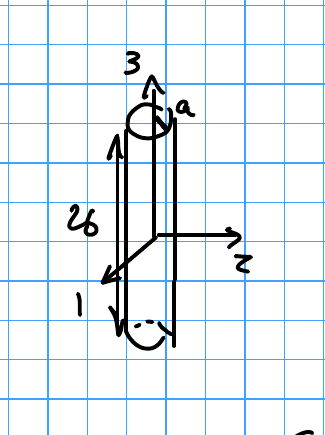
\includegraphics[width=\linewidth]{figures/rot_p5_rod.png}
\end{minipage}\hfill
\begin{minipage}{0.48\textwidth}\centering
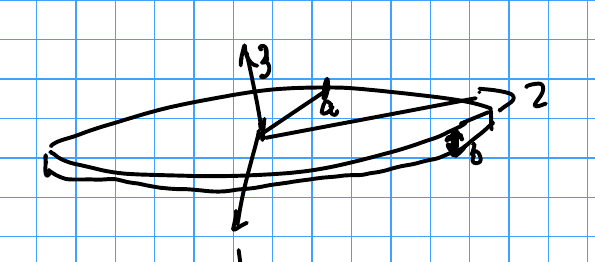
\includegraphics[width=\linewidth]{figures/rot_p5_disc.png}
\end{minipage}
\caption{Left: long thin rod of radius $a$ and length $2b$ about the body axes $1,2,3$;
$a\ll b \Rightarrow I_1 = I_2 > I_3$. Right: flat disc, $a\gg b \Rightarrow I_1 = I_2 < I_3$.}
\end{figure}

\begin{equation*}
I = \sum_P m_P\,\bigl(\text{distance to axis}\bigr)_P^{2} = \sum_P m_P\, r_{P\perp}^{2}
\end{equation*}
\begin{equation*}
I_3 \sim \mstruck{\,\#\,}\, M a^{2}
\qquad\qquad
I_1 \sim \mstruck{\,\#\,}\, M b^{2}
\end{equation*}
\begin{equation*}
a \ll b \;\Longrightarrow\; I_3 \ll I_1
\qquad\qquad
a \gg b \;\Longrightarrow\; I_3 \gg I_1
\end{equation*}

\begin{caveat}
The numerical coefficient in front of $Ma^{2}$ and $Mb^{2}$ is struck out in the source and is
not legible. Only the scaling is asserted; no value has been supplied here.
\end{caveat}

\begin{equation*}
\boxed{
\begin{aligned}
I_{ij} &= \sum_P m_P\bigl[\delta_{ij}\,r_P^{2} - r_{Pi} r_{Pj}\bigr]\\[4pt]
I_{33} &= \sum_P m_P\bigl[\underbrace{\delta_{33}}_{1}\,r_P^{2} - r_{P3} r_{P3}\bigr]\\[4pt]
&\hphantom{={}}\; r_{P1}r_{P1} + r_{P2}r_{P2} + \mstruck{r_{P3}r_{P3}} - \mstruck{r_{P3}r_{P3}}
\;=\; r_{P\perp}^{2}\\[2pt]
&\hphantom{={}}\; x\,x \;+\; y\,y \;+\; z\,z \;-\;z\,z
\;=\; x^{2}+y^{2} \;=\; \rho^{2}
\end{aligned}}
\end{equation*}

More irregular: $I_1$, $I_2$, $I_3$ all different.

\begin{equation*}
\begin{pmatrix} I_1 & 0 & 0\\ 0 & I_2 & 0\\ 0 & 0 & I_3\end{pmatrix}
\;\longleftrightarrow\;
I_{ij} = I_i\,\delta_{ij}
\qquad
L_i = \sum_{j=1}^{3} I_{ij}\,\omega_j = \sum_{j=1}^{3} I_i\,\delta_{ij}\,\omega_j = I_i\,\omega_i
\end{equation*}
\begin{equation*}
\begin{pmatrix} L_1\\ L_2\\ L_3\end{pmatrix}
= \begin{pmatrix} I_1 & 0 & 0\\ 0 & I_2 & 0\\ 0 & 0 & I_3\end{pmatrix}
\begin{pmatrix}\omega_1\\ \omega_2\\ \omega_3\end{pmatrix}
= \begin{pmatrix} I_1\omega_1\\ I_2\omega_2\\ I_3\omega_3\end{pmatrix}
\end{equation*}
\begin{equation*}
T = \frac{1}{2}\,\vec{\omega}\cdot\vec{L}
= \frac{1}{2}\sum_{i=1}^{3}\omega_i L_i
= \frac{1}{2}\sum_{i=1}^{3}\omega_i I_i \omega_i
= \frac{1}{2}\sum_{i=1}^{3} I_i \omega_i^{2}
\end{equation*}
\begin{equation*}
\boxed{\;L_i = I_i\,\omega_i\;}
\qquad\qquad
\boxed{\;T = \frac{1}{2}\sum_{i=1}^{3} I_i\,\omega_i^{2}\;}
\end{equation*}

\bigskip\hrule\bigskip

\section*{Parallel Axis Theorem}
\src{6}

$\bigl(\bar{I}_{ij}$ M of I w.r.t.\ CM$\bigr)$
\begin{equation*}
\boxed{\;
\underset{\substack{\uparrow\\ \textsc{origin o}}}{I_{ij}}
\;=\;
\underset{\substack{\updownarrow\\ \textsc{origin cm}}}{\bar{I}_{ij}}
\;+\; M\bigl[\delta_{ij}\,a^{2} - a_i a_j\bigr]\;}
\end{equation*}
Elementary version: $I = \bar{I} + M d^{2}$.

\section*{Rotation w.r.t.\ an arbitrarily moving point}

No longer look at a point in the body fixed in space.
\begin{itemize}
\item \textsc{inertial frame}
\item \textsc{cm frame}
  $\begin{cases}\textsc{may not be inertial if } \ddot{\vec{R}}\neq\vec{0}\\
   \textsc{axes} \parallel \textsc{axes of inertial frame}\end{cases}$
\item \textsc{body frame}
  $\begin{cases}\textsc{origin at } \vec{R} \Rightarrow \textsc{noninertial if } \ddot{\vec{R}}\neq\vec{0}\\
   \textsc{axes } 1\,2\,3 \textsc{ rotating w.r.t.\ } 1_0\,2_0\,3_0\end{cases}$
\end{itemize}

\begin{figure}[htbp]
\centering
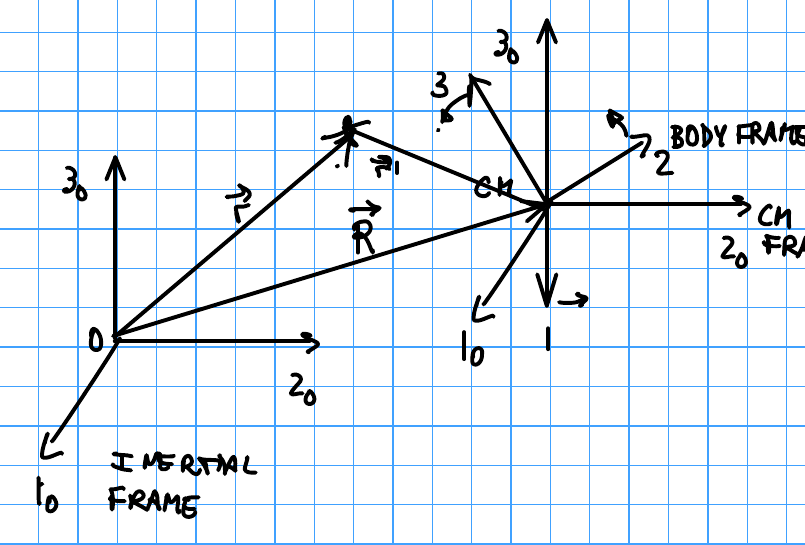
\includegraphics[width=0.78\textwidth]{figures/rot_p6_frames.png}
\caption{The three frames: inertial ($1_0\,2_0\,3_0$ at $O$), the CM frame (axes parallel to the
inertial ones), and the body frame ($1\,2\,3$, rotating with the body), with
$\vec{r} = \vec{R}+\vec{r}\,'$.}
\label{fig:frames}
\end{figure}

\begin{gather*}
\vec{r} = \vec{R} + \vec{r}\,'\\[4pt]
\left.\frac{\d\vec{r}}{\d t}\right|_{\textsc{inertial}}
= \frac{\d\vec{R}}{\d t} + \left.\frac{\d\vec{r}\,'}{\d t}\right|_{\textsc{cm}}
\end{gather*}
\begin{equation*}
\boxed{\;
\left.\frac{\d\vec{r}}{\d t}\right|_{\textsc{inertial}}
= \frac{\d\vec{R}}{\d t} + \left.\frac{\d\vec{r}\,'}{\d t}\right|_{\textsc{body}}
+ \vec{\omega}\times\vec{r}\,'\;}
\end{equation*}
\begin{equation*}
\boxed{\;
\textsc{if rigid body}\qquad
\left.\frac{\d\vec{r}}{\d t}\right|_{\textsc{inertial}}
= \frac{\d\vec{R}}{\d t} + \vec{\omega}\times\vec{r}\,'\;}
\end{equation*}

For any system of particles:
\begin{gather*}
M = \sum_P m_P
\qquad
\vec{R} \equiv \begin{array}{l}\textsc{center}\\ \textsc{of mass}\\ \textsc{position}\end{array}
\equiv \frac{\sum_P m_P \vec{r}_P}{\sum_P m_P}\\[6pt]
T = \tfrac{1}{2} M \dot{\vec{R}}^{2} + T' \qquad
T' = \sum_P \frac{m_P}{2}\,\dot{\vec{r}}\,'^{2}_P\\[4pt]
\vec{L} = \vec{R}\times M\dot{\vec{R}} + \vec{L}\,' \qquad
\vec{L}\,' = \sum_P \vec{r}\,'_P\times m_P\,\dot{\vec{r}}\,'_P
\end{gather*}
(the primed quantities are \textsc{measured in frame with origin at cm} --- the \textsc{cm frame}).

For rigid body $\dot{\vec{r}}\,'_P = \vec{\omega}\times\vec{r}\,'_P$:
\begin{align*}
\vec{L} &= \vec{R}\times M\dot{\vec{R}}
+ \underbrace{\sum_P \vec{r}\,'_P\times m_P\bigl(\vec{\omega}\times\vec{r}\,'_P\bigr)}_{\textsc{calculated before}}
&&\qquad L'_i = \sum_j \bar{I}_{ij}\,\omega_j\\
T &= \tfrac{1}{2} M \bigl|\dot{\vec{R}}\bigr|^{2}
+ \underbrace{\sum_P \frac{m_P}{2}\bigl(\vec{\omega}\times\vec{r}\,'_P\bigr)^{2}}_{\textsc{calculated before}}
&&\qquad T' = \tfrac{1}{2}\sum_{ij}\bar{I}_{ij}\,\omega_i\omega_j
\end{align*}

\bigskip\hrule\bigskip

\section*{Euler's Equations}
\src{7}

\begin{equation*}
\frac{\d\vec{L}}{\d t} = \vec{N}
\quad
\textsc{if}\;
\left\{
\begin{array}{l}
\times\ \textsc{inertial frame}\\
\times\ \textsc{cm frame (origin at cm may be}\\
\phantom{\times\ }\ \textsc{accelerated but it stays parallel}\\
\phantom{\times\ }\ \textsc{to inertial frame)}
\end{array}\right\}
\Leftrightarrow
\begin{array}{l}\text{``\textsc{translated}}\\ \textsc{but not rotated''}\end{array}
\end{equation*}
\begin{equation*}
\vec{N} = \frac{\d\vec{L}}{\d t}
= \left.\frac{\d\vec{L}}{\d t}\right|_{\textsc{body}} + \vec{\omega}\times\vec{L}
\end{equation*}
\begin{align*}
N_1 &= \left.\frac{\d L_1}{\d t}\right|_{\textsc{body}} + \bigl(\vec{\omega}\times\vec{L}\bigr)_1
= \left.\frac{\d L_1}{\d t}\right|_{\textsc{body}} + \omega_2 L_3 - \omega_3 L_2
\end{align*}
with $L_i = I_i\omega_i$ and $\left.\dot{I}_i\right|_{\textsc{body}} = 0$
(rigid body $\Rightarrow \dot{\vec{r}}_P = \vec{0}$ in body frame
$\Rightarrow \left.\dot{I}_i\right|_{\textsc{body}} = 0$):
\begin{equation*}
N_1 = I_1\left.\frac{\d\omega_1}{\d t}\right|_{\textsc{body}} + \omega_2 I_3\omega_3 - \omega_3 I_2\omega_2
= I_1\left.\frac{\d\omega_1}{\d t}\right|_{\textsc{body}} + \omega_2\omega_3\bigl(I_3-I_2\bigr)
\end{equation*}
\begin{equation*}
\boxed{
\begin{aligned}
I_1\left.\frac{\d\omega_1}{\d t}\right|_{\textsc{body}} &= \omega_2\omega_3\bigl(I_2-I_3\bigr) + N_1\\[4pt]
I_2\left.\frac{\d\omega_2}{\d t}\right|_{\textsc{body}} &= \omega_3\omega_1\bigl(I_3-I_1\bigr) + N_2\\[4pt]
I_3\left.\frac{\d\omega_3}{\d t}\right|_{\textsc{body}} &= \omega_1\omega_2\bigl(I_1-I_2\bigr) + N_3
\end{aligned}}
\qquad
\begin{array}{l}\textsc{euler's}\\ \textsc{equations}\end{array}
\end{equation*}

\section*{Applications: Kater's Pendulum}

\begin{figure}[htbp]
\centering
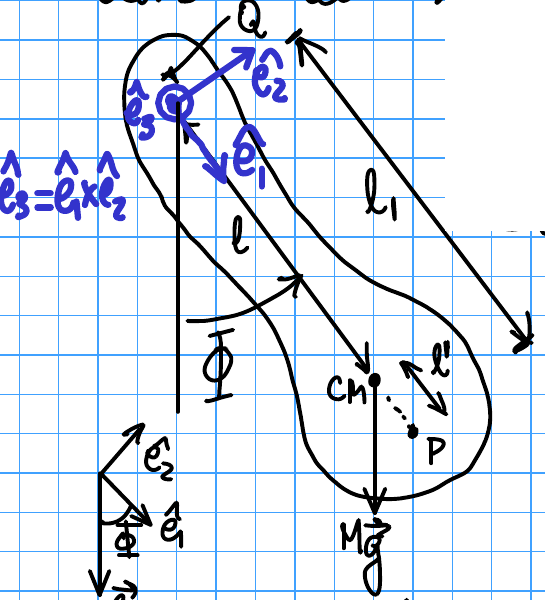
\includegraphics[width=0.42\textwidth]{figures/rot_p7_kater.png}
\caption{Kater's pendulum. Suspension point $Q$; body triad
$\ehat{1},\ehat{2},\ehat{3}=\ehat{1}\times\ehat{2}$ (blue); $l$ from $Q$ to the CM,
$l_1$ to the percussion centre $P$ at $l'$ beyond the CM; generalized coordinate $\bar{\Phi}$.}
\end{figure}

$n=1$ degree of freedom $\Longleftrightarrow$ angle $\bar{\Phi}\equiv$ gen coord.
\textsc{no friction}. $\omega_3 = \dot{\bar{\Phi}}$.

In Lab frame:
\begin{gather*}
I\,\dot{\omega}_3 = \frac{\d L_3}{\d t} = N_3 = -M g l \sin\bar{\Phi}\\[4pt]
\vec{N}_g = l\,\ehat{1}\times M\vec{g}
= l\,\ehat{1}\times M g\bigl(\cos\bar{\Phi}\,\ehat{1} - \sin\bar{\Phi}\,\ehat{2}\bigr)
= -M g l \sin\bar{\Phi}\;\ehat{3}\\[4pt]
\vec{g} = g\bigl(\cos\bar{\Phi}\,\ehat{1} - \sin\bar{\Phi}\,\ehat{2}\bigr)
\end{gather*}
\textsc{small angle} $\sin\bar{\Phi}\approx\bar{\Phi}$:
\begin{equation*}
I\,\ddot{\bar{\Phi}} \approx -M g l\,\bar{\Phi}
\qquad
\ddot{\bar{\Phi}} \approx -\frac{Mgl}{I}\,\bar{\Phi}
\qquad
\ddot{\bar{\Phi}} = -\Omega^{2}\,\bar{\Phi}
\qquad
\Omega = \Bigl(\frac{Mgl}{I}\Bigr)^{1/2}\ \text{\textsc{freq. of oscillation}}
\end{equation*}

\bigskip\hrule\bigskip

\subsection*{Parallel axis theorem}
\src{8}

\begin{equation*}
I = \bar{I} + M l^{2} = M\bar{k}^{2} + M l^{2} = M\bigl(\bar{k}^{2}+l^{2}\bigr) = M k^{2}
\end{equation*}
\textsc{define radius of gyration} $k$ \textsc{by} $I\equiv M k^{2}$;
\textsc{define} $\displaystyle l_1 \equiv \frac{k^{2}}{l} = l + \frac{\bar{k}^{2}}{l}$.

\begin{equation*}
\Omega_Q^{2} = \frac{\mstruck{M}\,g\,l}{\mstruck{M}\,\mstruck{\bigl(\bar{k}^{2}+l^{2}\bigr)}}
= \frac{g}{l_1}
\qquad\qquad
\bigl[\Omega^{2}\bigr] = \frac{\mstruck{L}/T^{2}}{\mstruck{L}} = \frac{1}{T^{2}}
\;\Longrightarrow\;
\bigl[\Omega\bigr] = \frac{1}{T}
\end{equation*}

\textsc{compare with simple pendulum} $\Omega = \sqrt{g/l}$ (point mass):
\begin{equation*}
\bar{I} = 0 \;\Longrightarrow\; \bar{k} = 0
\qquad
l_1 = l + \frac{\bar{k}^{2}}{l} = l
\end{equation*}
\begin{equation*}
\bar{I} = \int \d^{3}r\;\rho(\vec{r})\,\bigl(r_1^{2}+r_2^{2}\bigr)
\qquad
\begin{array}{l}\uparrow\ \uparrow\\ \text{distances measured w.r.t.\ CM}\end{array}
\end{equation*}
(for a point mass $r_1 = r_2 = 0$)
\begin{equation*}
\bar{k}^{2} = \frac{\bar{I}}{M}
= \frac{\displaystyle\int \d^{3}r\;\rho(\vec{r})\,\bigl(r_1^{2}+r_2^{2}\bigr)}{\displaystyle\int \d^{3}r\;\rho(\vec{r})}
\;\Longleftrightarrow\;
\begin{array}{l}\text{Average squared distance to axis of rotation}\\
\text{weighted by the mass density }\rho(\vec{r})\end{array}
\end{equation*}

Suspend the pendulum from point $P$ (``Percussion center'') at distance $l_1$ from $Q_1$
along the direction that goes through CM:
\begin{equation*}
\Omega_Q^{2} = \frac{\mstruck{M}\,g\,l}{\mstruck{M}\,\mstruck{\bigl(\bar{k}^{2}+l^{2}\bigr)}} = \frac{g}{l_1}
\qquad
\Omega_P^{2} = \frac{g\,l'}{\bar{k}^{2}+l'^{2}}
= \frac{g\,(l_1-l)}{\bar{k}^{2}+(l_1-l)^{2}}
= \frac{g\,\bar{k}^{2}/l}{\bar{k}^{2}+\bar{k}^{4}/l^{2}}
= \frac{g\,l}{l^{2}+\bar{k}^{2}} = \Omega_Q^{2}
\end{equation*}
\begin{equation*}
l_1 = l + \frac{\bar{k}^{2}}{l}
\qquad
l_1 - l = \frac{\bar{k}^{2}}{l}
\qquad
\bigl(l_1-l\bigr)^{2} = \frac{\bar{k}^{4}}{l^{2}}
\end{equation*}

\bigskip\hrule\bigskip

\section*{Torque-Free Motion in 3D: Symmetric Top}

$I_1 = I_2 \neq I_3$, \qquad $\displaystyle \Omega \equiv \omega_3\,\frac{I_3-I_1}{I_1}$.
\begin{align*}
I_1\left.\frac{\d\omega_1}{\d t}\right|_{\textsc{body}} = \omega_2\omega_3\bigl(I_2-I_3\bigr)
&\;\Longrightarrow\; \dot{\omega}_1 = -\Bigl[\omega_3\,\frac{I_3-I_2}{I_1}\Bigr]\omega_2\\
I_2\left.\frac{\d\omega_2}{\d t}\right|_{\textsc{body}} = \omega_3\omega_1\bigl(I_3-I_1\bigr)
&\;\Longrightarrow\; \dot{\omega}_2 = \Bigl[\omega_3\,\frac{I_3-I_1}{I_2}\Bigr]\omega_1\\
I_3\left.\frac{\d\omega_3}{\d t}\right|_{\textsc{body}} = \omega_1\omega_2\bigl(I_1-I_2\bigr)
&\;\Longrightarrow\;
\end{align*}
\begin{equation*}
\boxed{
\begin{aligned}
\dot{\omega}_1 &= -\Omega\,\omega_2\\
\dot{\omega}_2 &= \Omega\,\omega_1\\
\dot{\omega}_3 &= 0
\end{aligned}}
\end{equation*}

\bigskip\hrule\bigskip

\src{9}
\begin{equation*}
\dot{\vec{\omega}} = \Omega\,\ehat{3}\times\vec{\omega}
\quad\Longleftrightarrow\quad
\vec{\omega}\ \text{rotates with angular velocity}\ \Omega\,\ehat{3}
\;\Longrightarrow\; \textsc{precession}
\end{equation*}
\begin{gather*}
\dot{\vec{\omega}} = \Omega\,\ehat{3}\times\vec{\omega}
= \Omega\,\ehat{3}\times\bigl(\omega_1\ehat{1}+\omega_2\ehat{2}+\omega_3\ehat{3}\bigr)
= \Omega\bigl(\omega_1\ehat{2} - \omega_2\ehat{1}\bigr)\\[4pt]
\dot{\omega}_1 = -\Omega\,\omega_2 \qquad \dot{\omega}_2 = \Omega\,\omega_1 \qquad \dot{\omega}_3 = 0
\end{gather*}
$\vec{\omega}$ rotates around $\ehat{3}$ with ang.\ speed $\Omega$.
If initially $\vec{\omega} = \omega\bigl(\sin\lambda\,\ehat{1} + \cos\lambda\,\ehat{3}\bigr)$,
then $\vec{\omega}\in$ plane of $\ehat{1}$ and $\ehat{3}$:
\begin{equation*}
\boxed{\;
\omega_1 = \omega\sin\lambda\,\cos(\Omega t)
\qquad
\omega_2 = \omega\sin\lambda\,\sin(\Omega t)
\qquad
\omega_3 = \omega\cos\lambda\;}
\end{equation*}

\begin{figure}[htbp]
\centering
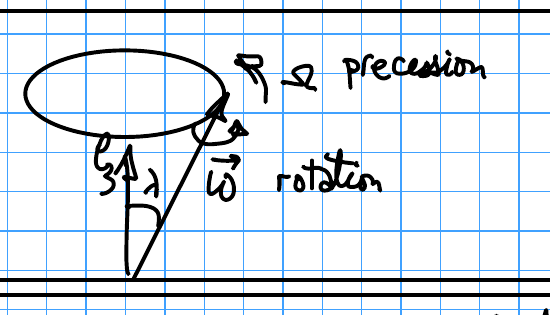
\includegraphics[width=0.45\textwidth]{figures/rot_p9_cone.png}
\caption{$\vec{\omega}$ (rotation) sweeps a cone of half-angle $\lambda$ about the body axis
$\ehat{3}$ at the precession rate $\Omega$.}
\end{figure}

\bigskip\hrule\bigskip

\section*{Euler Angles}

$\ezero{1}\,\ezero{2}\,\ezero{3}$ \textsc{inertial set of unit vectors (not rotating)};
$\ehat{1}\,\ehat{2}\,\ehat{3}$ \textsc{body set of unit vectors (rotating with body)}.
The three-frame construction of Figure~\ref{fig:frames} is redrawn here.

\begin{quote}
\textbf{Following Ch5 F\&W (Skipping a lot)}
\end{quote}

We need 6 coordinates to describe positions of all points in a \textsc{rigid body}:
\begin{itemize}
\item \textsc{cm position} $\vec{R} \Longleftrightarrow X\,Y\,Z$;
\item 3 coord to fix orientation of $\ehat{1}\ehat{2}\ehat{3}$ w.r.t.\ $\ezero{1}\ezero{2}\ezero{3}$.
\end{itemize}
\textsc{we choose euler angles:} $\alpha,\beta,\gamma$.
\begin{itemize}
\item $\ehat{\beta} \perp \ezero{3},\,\ehat{3}$
\item \textsc{orientation of new north pole} $\longrightarrow$ $\beta$ \textsc{polar},
      $\alpha$ \textsc{azimuthal}
\item $\gamma$ \textsc{specifies additional rotation around} $\ehat{3}$
\item $\alpha,\beta,\gamma$ \textsc{can be chosen independently and they completely specify
      orientation of body frame} $\Longrightarrow$
      \textcolor{lecred}{\textsc{use} $\alpha$ $\beta$ $\gamma$ \textsc{as generalized coord}}
\end{itemize}

\begin{figure}[htbp]
\centering
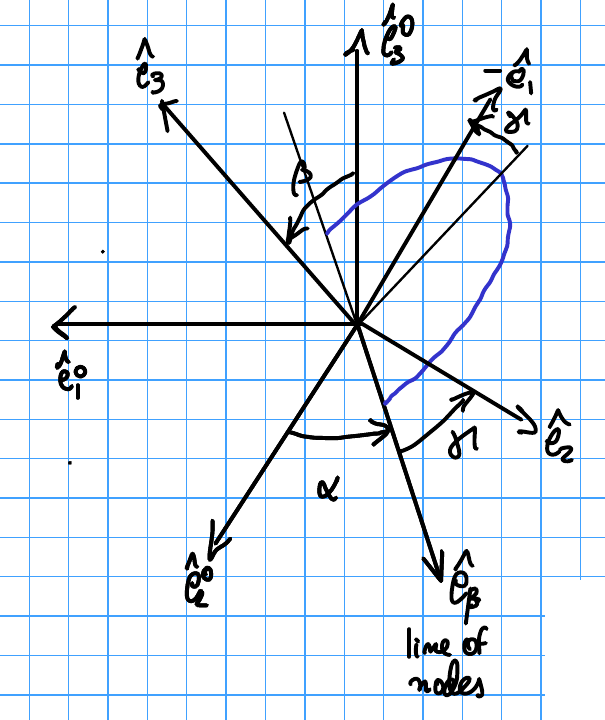
\includegraphics[width=0.52\textwidth]{figures/rot_p9_euler.png}
\caption{Definition of the Euler angles. Space triad $\ezero{1},\ezero{2},\ezero{3}$; body triad
$\ehat{1},\ehat{2},\ehat{3}$ (note $-\ehat{1}$ as drawn); $\alpha$ azimuthal, $\beta$ polar,
$\gamma$ the additional rotation about $\ehat{3}$; $\ehat{\beta}$ is the line of nodes.}
\end{figure}

\begin{gather*}
\textcolor{lecgreen}{T = \tfrac{1}{2}\bigl(I_1\omega_1^{2} + I_2\omega_2^{2} + I_3\omega_3^{2}\bigr)}
\tag{1}\label{eq:B1}\\[4pt]
\textcolor{lecgreen}{\vec{\omega} = \dot{\alpha}\,\ezero{3} + \dot{\beta}\,\ehat{\beta} + \dot{\gamma}\,\ehat{3}}
\tag{2}\label{eq:B2}\\[4pt]
\textcolor{lecgreen}{\ehat{\beta} = \cos\gamma\,\ehat{2} + \sin\gamma\,\ehat{1}}
\tag{3}\label{eq:B3}\\[4pt]
\textcolor{lecgreen}{\ezero{3} = \cos\beta\,\ehat{3}
+ \sin\beta\bigl[\cos\gamma\,(-\ehat{1}) + \sin\gamma\,\ehat{2}\bigr]}
\tag{4}\label{eq:B4}
\end{gather*}
\begin{equation*}
\boxed{\textcolor{lecgreen}{\;
\vec{\omega} = \bigl(-\dot{\alpha}\sin\beta\cos\gamma + \dot{\beta}\sin\gamma\bigr)\ehat{1}
+ \bigl(\dot{\alpha}\sin\beta\sin\gamma + \dot{\beta}\cos\gamma\bigr)\ehat{2}
+ \bigl(\dot{\gamma} + \dot{\alpha}\cos\beta\bigr)\ehat{3}\;}}
\tag{5}\label{eq:B5}
\end{equation*}

\bigskip\hrule\bigskip

\src{10}
\textcolor{lecgreen}{\textsc{note}: Infinitesimal rot.}
\begin{align*}
\textcolor{lecgreen}{R_\alpha} &\textcolor{lecgreen}{{}= \mathbf{1} + M_\alpha\,\dot{\alpha}\,\d t}
\tag{6}\label{eq:B6}\\
\textcolor{lecgreen}{R_\beta} &\textcolor{lecgreen}{{}= \mathbf{1} + M_\beta\,\dot{\beta}\,\d t}
\tag{7}\label{eq:B7}\\[4pt]
\textcolor{lecgreen}{R_\alpha R_\beta}
&\textcolor{lecgreen}{{}= \mathbf{1} + \bigl(M_\alpha\dot{\alpha}+M_\beta\dot{\beta}\bigr)\d t
+ \mstruck{\mathcal{O}\bigl((\d t)^{2}\bigr)}}
\tag{8}\label{eq:B8}\\
\textcolor{lecgreen}{R_\beta R_\alpha}
&\textcolor{lecgreen}{{}= \mathbf{1} + \bigl(M_\beta\dot{\beta}+M_\alpha\dot{\alpha}\bigr)\d t
+ \mstruck{\mathcal{O}\bigl((\d t)^{2}\bigr)}}
\tag{9}\label{eq:B9}\\[4pt]
&\textcolor{lecgreen}{\text{\textsc{equal to order} }\d t \text{ --- the }
\mathcal{O}\bigl((\d t)^{2}\bigr)\text{ terms are struck out}}
\end{align*}

\begin{equation*}
\textcolor{lecgreen}{\Longrightarrow\ \textsc{infinitesimal rotations add},\qquad
\vec{\omega} = \vec{\omega}_\alpha + \vec{\omega}_\beta + \vec{\omega}_\gamma}
\tag{10}\label{eq:B10}
\end{equation*}
\hfill$\eqref{eq:B10} \Longrightarrow \eqref{eq:B2}$

\subsection*{Kinetic energy --- General case}

\begin{equation*}
\boxed{\;
\begin{aligned}
T &= \frac{I_1}{2}\omega_1^{2} + \frac{I_2}{2}\omega_2^{2} + \frac{I_3}{2}\omega_3^{2}\\
&= \frac{I_1}{2}\bigl(-\dot{\alpha}\sin\beta\cos\gamma + \dot{\beta}\sin\gamma\bigr)^{2}
+ \frac{I_2}{2}\bigl(\dot{\alpha}\sin\beta\sin\gamma + \dot{\beta}\cos\gamma\bigr)^{2}
+ \frac{I_3}{2}\bigl(\dot{\gamma}+\dot{\alpha}\cos\beta\bigr)^{2}
\end{aligned}\;}
\tag{11}\label{eq:B11}
\end{equation*}
\begin{equation*}
\text{Symmetric Top:}\qquad I_1 = I_2 \tag{12}\label{eq:B12}
\end{equation*}
\begin{equation*}
\boxed{\;
T = \frac{I_1}{2}\bigl(\dot{\beta}^{2} + \dot{\alpha}^{2}\sin^{2}\beta\bigr)
+ \frac{I_3}{2}\bigl(\dot{\gamma}+\dot{\alpha}\cos\beta\bigr)^{2}\;}
\tag{13}\label{eq:B13}
\end{equation*}

\subsection*{Torque-Free Motion of symmetric top}

\begin{equation*}
\boxed{\;
L = T = \frac{I_1}{2}\bigl(\dot{\beta}^{2} + \dot{\alpha}^{2}\sin^{2}\beta\bigr)
+ \frac{I_3}{2}\bigl(\dot{\gamma}+\dot{\alpha}\cos\beta\bigr)^{2}\;}
\tag{14}\label{eq:B14}
\end{equation*}

$\alpha,\beta,\gamma$ Gen Coord $\Longrightarrow$ 3 Lagrange Eqns.
\begin{equation*}
\text{\textsc{2 cyclic coordinates}: } \alpha,\ \gamma \tag{15}\label{eq:B15}
\end{equation*}
$\Longrightarrow$ 2 \textsc{const of motion}:
\begin{align*}
p_\alpha &= \pd{L}{\dot{\alpha}}
= I_1 \sin^{2}\!\beta\;\dot{\alpha} + I_3\bigl(\dot{\gamma}+\dot{\alpha}\cos\beta\bigr)\cos\beta
\tag{16}\label{eq:B16}\\[4pt]
p_\gamma &= \pd{L}{\dot{\gamma}} = I_3\bigl(\dot{\gamma}+\dot{\alpha}\cos\beta\bigr)
\tag{17}\label{eq:B17}
\end{align*}

\begin{equation*}
\fbox{$\displaystyle
\begin{array}{l}
\textsc{we will show later that:}\\[6pt]
\qquad p_\alpha = \vec{L}\cdot\ezero{3} \hfill \eqref{eq:B18}\\[6pt]
\qquad p_\gamma = \vec{L}\cdot\ehat{3} \hfill \eqref{eq:B19}
\end{array}$}
\end{equation*}

We compute now
\begin{equation*}
p_\gamma = \pd{L}{\dot{\gamma}} = I_3\bigl(\dot{\gamma}+\dot{\alpha}\cos\beta\bigr)
\tag*{\eqref{eq:B17}}
\end{equation*}
and notice that, using \eqref{eq:B5},
\begin{equation*}
\boxed{\;p_\gamma = I_3\,\omega_3 = \vec{L}\cdot\ehat{3}\;}\quad\checkmark
\qquad \text{\textsc{as anticipated}}
\tag{19}\label{eq:B19}
\end{equation*}
Also
\begin{equation*}
p_\alpha = \pd{L}{\dot{\alpha}}
= I_1\sin^{2}\!\beta\;\dot{\alpha} + I_3\bigl(\dot{\gamma}+\dot{\alpha}\cos\beta\bigr)\cos\beta
\tag*{\eqref{eq:B16}}
\end{equation*}
\begin{equation*}
\textcolor{lecgreen}{\vec{L} = I_1\bigl(\omega_1\ehat{1} + \omega_2\ehat{2}\bigr) + I_3\,\omega_3\,\ehat{3}}
\tag{20}\label{eq:B20}
\end{equation*}
Compare with
\begin{align*}
\vec{L}\cdot\ezero{3}
&= \overbrace{\textcolor{lecgreen}{\Bigl(I_1\bigl(\omega_1\ehat{1}+\omega_2\ehat{2}\bigr)+I_3\omega_3\ehat{3}\Bigr)}}^{\eqref{eq:B20}}
\cdot
\overbrace{\Bigl(\cos\beta\,\ehat{3}+\sin\beta\bigl[\cos\gamma(-\ehat{1})+\sin\gamma\,\ehat{2}\bigr]\Bigr)}^{\eqref{eq:B4}}
\tag{21}\label{eq:B21}\\[6pt]
&= I_1\Bigl[\bigl(-\dot{\alpha}\sin\beta\cos\gamma+\dot{\beta}\sin\gamma\bigr)\bigl(-\sin\beta\cos\gamma\bigr)
+ \bigl(\dot{\alpha}\sin\beta\sin\gamma+\dot{\beta}\cos\gamma\bigr)\bigl(\sin\beta\sin\gamma\bigr)\Bigr]\\
&\qquad + I_3\bigl(\dot{\gamma}+\dot{\alpha}\cos\beta\bigr)\cos\beta
\tag{22}\label{eq:B22}\\[6pt]
&= I_1\,\dot{\alpha}\,\sin^{2}\!\beta\bigl(\cos^{2}\gamma+\sin^{2}\gamma\bigr)
+ I_3\bigl(\dot{\gamma}+\dot{\alpha}\cos\beta\bigr)\cos\beta
\tag{23}\label{eq:B23}
\end{align*}
\begin{equation*}
\boxed{\;
\vec{L}\cdot\ezero{3} = I_1\,\dot{\alpha}\,\sin^{2}\!\beta
+ I_3\bigl(\dot{\gamma}+\dot{\alpha}\cos\beta\bigr)\cos\beta = p_\alpha \;}\quad\checkmark
\tag{18}\label{eq:B18}
\end{equation*}

\bigskip\hrule\bigskip

\src{11}
\begin{equation*}
p_\beta = \pd{L}{\dot{\beta}} = I_1\,\dot{\beta}
\tag{24}\label{eq:B24}
\end{equation*}
\textsc{not a constant (in principle) because} $\beta$ \textsc{appears explicitly in the lagrangian}.
\begin{equation*}
\pd{L}{\beta} = I_1\sin\beta\cos\beta\;\dot{\alpha}^{2}
- I_3\bigl(\dot{\gamma}+\dot{\alpha}\cos\beta\bigr)\dot{\alpha}\sin\beta
= \dot{\alpha}\sin\beta\bigl(I_1\dot{\alpha}\cos\beta - I_3\omega_3\bigr)
\tag{25}\label{eq:B25}
\end{equation*}
Then
\begin{equation*}
\boxed{\;
\dot{p}_\beta = \pd{L}{\beta} = \dot{\alpha}\sin\beta\bigl(I_1\dot{\alpha}\cos\beta - I_3\omega_3\bigr)\;}
\qquad (\text{However, see later})
\tag{26}\label{eq:B26}
\end{equation*}

Compare $p_\beta$ with
\begin{equation*}
\vec{L}\cdot\ehat{\beta}
= \overbrace{\textcolor{lecgreen}{\Bigl(I_1\bigl(\omega_1\ehat{1}+\omega_2\ehat{2}\bigr)+I_3\omega_3\ehat{3}\Bigr)}}^{\eqref{eq:B20}}
\cdot
\overbrace{\textcolor{lecgreen}{\bigl(\cos\gamma\,\ehat{2}+\sin\gamma\,\ehat{1}\bigr)}}^{\eqref{eq:B3}}
\end{equation*}
Recall
\begin{equation*}
\textcolor{lecgreen}{\vec{\omega} = \bigl(-\dot{\alpha}\sin\beta\cos\gamma+\dot{\beta}\sin\gamma\bigr)\ehat{1}
+ \bigl(\dot{\alpha}\sin\beta\sin\gamma+\dot{\beta}\cos\gamma\bigr)\ehat{2}
+ \bigl(\dot{\gamma}+\dot{\alpha}\cos\beta\bigr)\ehat{3}}
\tag*{\eqref{eq:B5}}
\end{equation*}
\begin{align*}
\vec{L}\cdot\ehat{\beta}
&= I_1\Bigl[\bigl(-\dot{\alpha}\sin\beta\cos\gamma+\dot{\beta}\sin\gamma\bigr)\sin\gamma
+ \bigl(\dot{\alpha}\sin\beta\sin\gamma+\dot{\beta}\cos\gamma\bigr)\cos\gamma\Bigr]
\tag{27}\label{eq:B27}\\[4pt]
&= I_1\,\dot{\beta}\bigl(\sin^{2}\gamma+\cos^{2}\gamma\bigr) = I_1\,\dot{\beta}
\tag{28}\label{eq:B28}
\end{align*}
\begin{equation*}
\Longrightarrow\quad
\boxed{\;\vec{L}\cdot\ehat{\beta} = p_\beta\;}\quad\checkmark
\tag{29}\label{eq:B29}
\end{equation*}

\subsection*{Description in Inertial (or CM) Frame}

\begin{gather*}
\text{No torque} \tag{30}\label{eq:B30}\\
\dot{\vec{L}} = \vec{0} \tag{31}\label{eq:B31}
\end{gather*}
\begin{equation*}
\Longleftrightarrow\;
\left\{
\begin{array}{l@{\qquad}l}
\textsc{choose } \ezero{3} \parallel \vec{L} & (32)\\[4pt]
\bigl|\vec{L}\bigr| \text{ doesn't change} & (33)
\end{array}\right.
\end{equation*}
\begin{align*}
\Longrightarrow\qquad &\vec{L}\cdot\ezero{3} = \bigl|\vec{L}\bigr|
\tag{34}\label{eq:B34}\\
\text{\textsc{and}}\qquad &\vec{L} = \bigl|\vec{L}\bigr|\,\ezero{3}
\tag{35}\label{eq:B35}
\end{align*}

We know that $\vec{L}\cdot\ehat{3} = p_\gamma$ is a constant of the motion:
\begin{equation*}
\underbrace{\vec{L}\cdot\ehat{3}}_{\substack{=\,p_\gamma\\ =\,\textsc{const}}}
= \underbrace{\bigl|\vec{L}\bigr|}_{=\,\textsc{const}}\;\ezero{3}\cdot\ehat{3}
\tag{36}\label{eq:B36}
\end{equation*}
\begin{equation*}
\Longrightarrow\quad \ezero{3}\cdot\ehat{3}\ \textsc{constant}
\tag{37}\label{eq:B37}
\end{equation*}
\begin{equation*}
\textsc{const} = \ezero{3}\cdot\ehat{3}
= \cos\bigl(\text{angle between } \ehat{3} \text{ and } \ezero{3}\bigr) = \cos\beta
\tag{38}\label{eq:B38}
\end{equation*}
\begin{align*}
&\beta \ \textsc{is a constant of the motion}
\tag{39}\label{eq:B39}\\
\Longrightarrow\quad &\dot{\beta} = 0
\tag{40}\label{eq:B40}
\end{align*}
\begin{equation*}
\Longrightarrow\quad
\boxed{\;p_\beta = I_1\,\dot{\beta} = \vec{L}\cdot\ehat{\beta} = 0\;}
\tag{41}\label{eq:B41}
\end{equation*}

\hfill\textit{[margin: For this particular choice of axes, $p_\beta$ and $\vec{L}\cdot\ehat{\beta}$
are zero!!]}

\begin{align*}
\left.\begin{aligned}
&\vec{L}\cdot\ehat{\beta} = 0 &&\eqref{eq:B41}\\
&\vec{L} \neq 0,\quad \bigl|\ehat{\beta}\bigr| = 1 \neq 0
\end{aligned}\right\}
\;&\Longrightarrow\;
\vec{L} \perp \ehat{\beta}
\tag{42}\label{eq:B42}\\
&\Longrightarrow\;
\boxed{\;\vec{L}\ \text{is in the plane of}\ \ehat{3}\ \text{and}\ \ezero{3}\;}
\tag{43}\label{eq:B43}
\end{align*}

\bigskip

\textsc{constants:} $I_1$, $I_3$, $\beta$, $I_3\omega_3 = L_3$, $p_\alpha$.
\begin{equation*}
p_\alpha = \pd{L}{\dot{\alpha}}
= \underbrace{I_1\sin^{2}\!\beta\;\dot{\alpha}
+ I_3\bigl(\dot{\gamma}+\dot{\alpha}\cos\beta\bigr)\cos\beta}_{\eqref{eq:B16}}
\;\underset{\eqref{eq:B5}}{=}\;
\underline{I_1}\;\underline{\sin^{2}\!\beta}\;\dot{\alpha} + \underline{I_3\omega_3}\;\underline{\cos\beta}
\tag{44}\label{eq:B44}
\end{equation*}
\begin{equation*}
\Longrightarrow\quad \boxed{\;\dot{\alpha}\ \textsc{constant}\;}
\tag{45}\label{eq:B45}
\end{equation*}
\begin{equation*}
\left.\begin{aligned}
&p_\gamma = \pd{L}{\dot{\gamma}} = I_3\bigl(\dot{\gamma}+\dot{\alpha}\cos\beta\bigr)
&&\eqref{eq:B17}\\
&I_3,\ p_\gamma,\ \dot{\alpha},\ \beta\ \textsc{constant}
\end{aligned}\right\}
\;\Longrightarrow\;
\boxed{\;\dot{\gamma}\ \textsc{constant}\;}
\tag{46}\label{eq:B46}
\end{equation*}
\begin{align*}
\alpha &= \dot{\alpha}_0\,t \tag{47}\label{eq:B47}\\
\gamma &= \dot{\gamma}_0\,t \tag{48}\label{eq:B48}
\end{align*}
\hfill $\dot{\alpha}_0,\ \dot{\gamma}_0$ \textsc{constants}

\bigskip\hrule\bigskip

\src{12}
\begin{equation*}
0 \overset{\eqref{eq:B41}}{=} \dot{p}_\beta
= \overset{\eqref{eq:B26}}{\pd{L}{\beta}}
= \dot{\alpha}\sin\beta\bigl(I_1\dot{\alpha}\cos\beta - I_3\omega_3\bigr)
\;\Longrightarrow\;
\boxed{\;\dot{\alpha}\cos\beta = \frac{I_3\,\omega_3}{I_1}\;}
\tag{49}\label{eq:B49}
\end{equation*}
\begin{equation*}
\eqref{eq:B5}\;\Longrightarrow\;
\omega_3 = \dot{\gamma}+\dot{\alpha}\cos\beta
\overset{\eqref{eq:B49}}{=} \dot{\gamma} + \frac{I_3}{I_1}\,\omega_3
\;\Longrightarrow\;
\boxed{\;\dot{\gamma} = \omega_3\,\frac{I_1-I_3}{I_1} = -\Omega\;}
\tag{51}\label{eq:B51}
\end{equation*}
\begin{equation*}
\Omega \equiv \omega_3\,\frac{I_3-I_1}{I_1}
\tag{50}\label{eq:B50}
\end{equation*}
\hfill\emph{defined when looking at body frame evolution of $\vec{\omega}$ a couple of lectures before}

\begin{figure}[htbp]
\centering
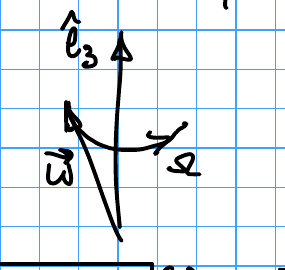
\includegraphics[width=0.20\textwidth]{figures/rot_p12_sketch.png}
\caption{$\vec{\omega}$ and the precession rate $\Omega$ relative to the body axis $\ehat{3}$.}
\end{figure}

\begin{align*}
\eqref{eq:B2} + \eqref{eq:B40}\;&\Longrightarrow\;
\boxed{\;\vec{\omega} = \dot{\alpha}\,\ezero{3} + \dot{\gamma}\,\ehat{3}\;}
\tag{52}\label{eq:B52}\\
&\Longrightarrow\;
\boxed{\;\ehat{3},\ \ezero{3},\ \vec{\omega},\ \vec{L}\ \text{are in one plane}\;}
\tag{53}\label{eq:B53}
\end{align*}

Consider cases where $I_1 = I_2 < I_3$ or $I_1 = I_2 > I_3$:
\begin{equation*}
\vec{L} = I_1\bigl(\omega_1\ehat{1} + \omega_2\ehat{2}\bigr) + I_3\,\omega_3\,\ehat{3}
\tag*{\eqref{eq:B20}}
\end{equation*}

\bigskip\hrule\bigskip

\begin{center}
\begin{tabular}{c@{\qquad\qquad}c}
\textsc{simple pendulum:} & \textsc{thumbtack:}\\[8pt]
$\displaystyle \ddot{\Theta} = -\frac{g}{l}\,\sin\Theta$
&
$\displaystyle \bigl(\text{angle}\bigr)^{\!\bm{\cdot\cdot}}
= -\left[\begin{array}{c}\textsc{awful}\\ \textsc{mess}\end{array}\right]\sin\bigl(\text{angle}\bigr)$
\end{tabular}
\end{center}

\hrule

\end{document}
